%! Author = Wiktor Rostkowski
%! Date = 13/06/2024

\chapter{Prezentacja systemu}
\label{ch:prezentacja-systemu}



\section{Widok głównej stron}
\label{sec:mapawidok}

Aplikacja prezentuje użytkownikom interaktywną mapę z zaznaczonymi atrakcjami turystycznymi (POI). 
Na głównym ekranie znajdują się różne elementy interfejsu, które ułatwiają nawigację~i~dostęp do kluczowych funkcji.

Główną część widoku aplikacji stanowi interaktywna mapa, na której zaznaczone są punkty zainteresowania. Użytkownicy mogą:
\begin{itemize}
 \item   Kliknąć na poszczególne POI, aby uzyskać więcej informacji~o~danej atrakcji.
 \item   Zaznaczać~i~dodawać POI do koszyka.
 \item  Korzystać z opcji wyznaczania tras pomiędzy wybranymi punktami.
\end{itemize}
Mapa jest interaktywna~i~responsywna, pozwalając użytkownikom na swobodne powiększanie, pomniejszanie oraz przesuwanie widoku~w~celu znalezienia interesujących miejsc.

\begin{figure}[H]
    \centering
    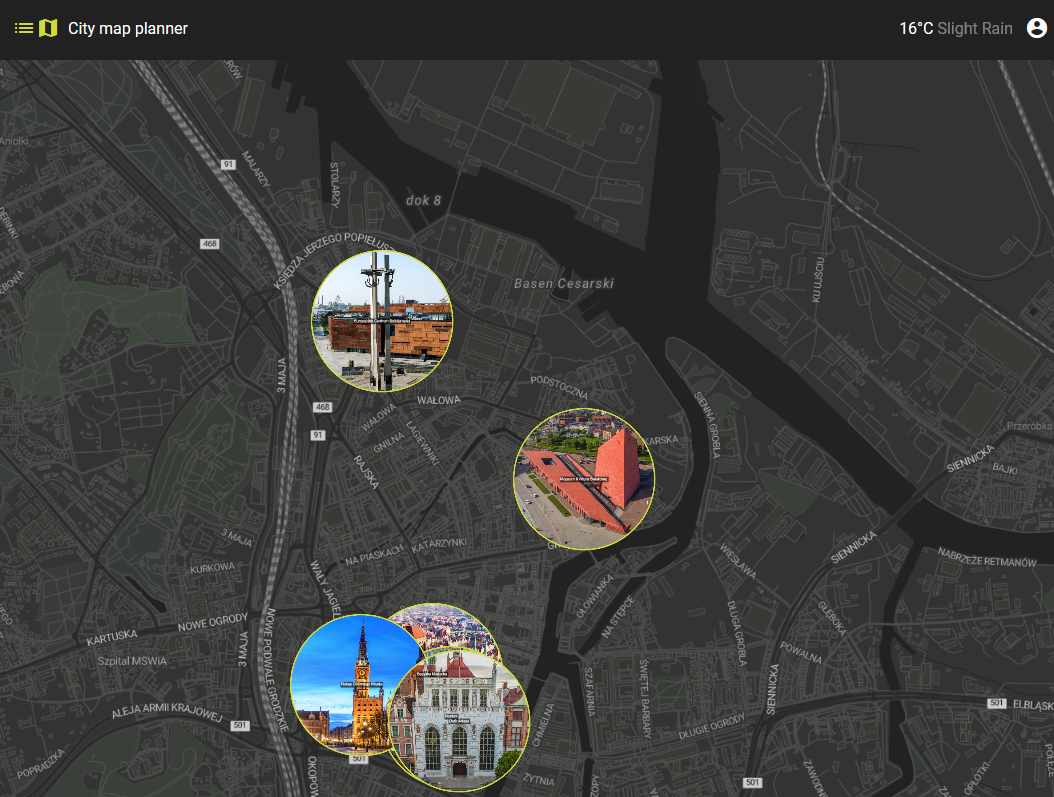
\includegraphics[width=1\textwidth]{attachments/mapawidok}
    \caption{Widok głównej strony}
    \label{fig:mapawidok}
    \end{figure}
    \begin{figure}[H]
        \centering
        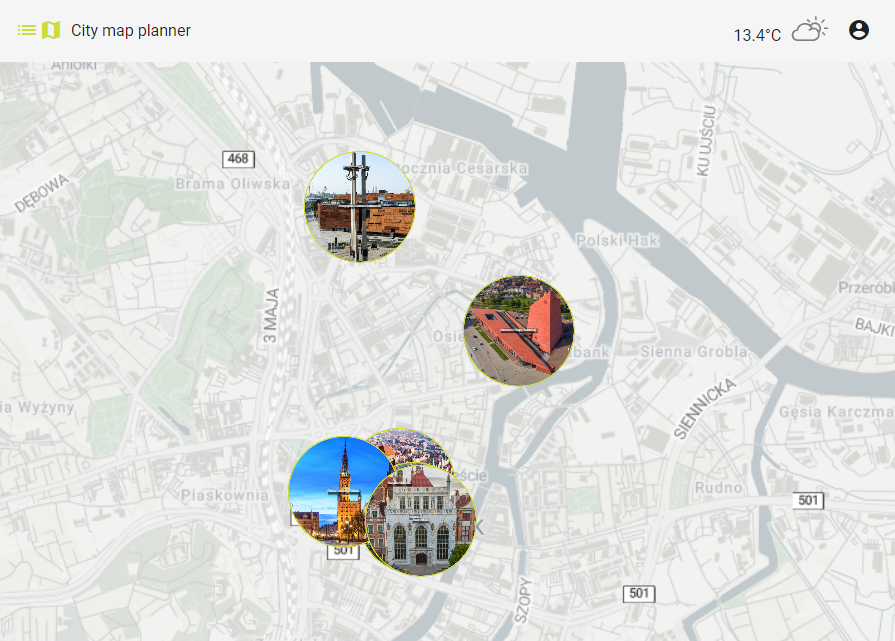
\includegraphics[width=1\textwidth]{attachments/mapawidok-light}
        \caption{Widok głównej strony wersja jasna}
        \label{fig:mapawidok1}
        \end{figure}
        \begin{figure}[H]
            \centering
            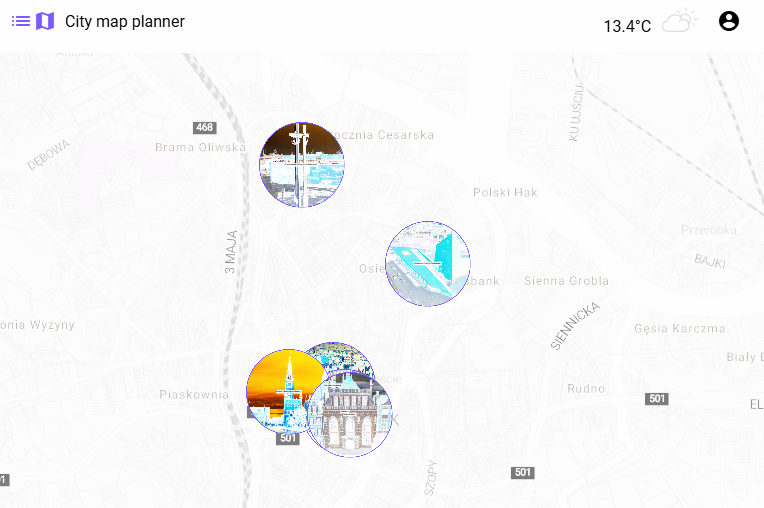
\includegraphics[width=1\textwidth]{attachments/mapawidok-high-contrast}
            \caption{Widok głównej strony wersja wysoki kontrast}
            \label{fig:mapawidok2}
            \end{figure}

\subsection{Pasek Nawigacji}
\label{sec:pasek-nawigacji}
Pasek główny z nawigacją znajduje się na górze ekranu, zapewniając szybki dostęp do najważniejszych sekcji aplikacji. Na pasku znajdują się następujące elementy:
\begin{itemize}
    \item link do listy POI;
    \item link do strony głównej;
    \item aktualna Temperatura;
    \item obok temperatury wyświetlana jest ikona pogody(np. deszcz, słońce), która wizualnie przedstawia obecne warunki atmosferyczne;
    \item jeśli użytkownik wybrał jakieś punkty zainteresowania, pojawia się link do koszyka;
    \item link do zarządzania konta użytkownika;
\end{itemize}
\begin{figure}[H]
    \centering
    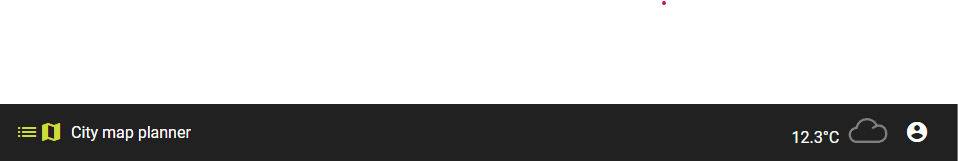
\includegraphics[width=1\textwidth]{attachments/nav-baner}
    \caption{Pasek Nawigacji}
    \label{fig:pasek-nawigacji}
\end{figure}

\section{Widok pojedynczej atrakcji}
\label{sec:atrakcjawidok}
Widok pojedynczej atrakcji~w~aplikacji został zaprojektowany tak, aby dostarczyć 
użytkownikom wszystkie niezbędne informacje~w~przejrzysty~i~estetyczny sposób. 
Składa się z kilku kluczowych elementów, które pomagają użytkownikowi zapoznać się z daną atrakcją oraz podjąć decyzję~o~jej odwiedzeniu.
\newline
Zdjęcie atrakcji:
Na samej górze ekranu znajduje się duże, wysokiej jakości zdjęcie atrakcji. 
Zdjęcie to pozwala użytkownikom wizualnie ocenić miejsce~i~zyskać wstępne wrażenie. Jest to pierwsza rzecz, którą widzą użytkownicy, co ma na celu przyciągnięcie ich uwagi~i~zainteresowanie.
\newline
Tytuł atrakcji:
Bezpośrednio pod zdjęciem znajduje się tytuł atrakcji. Jest to nazwa miejsca, która jest 
wyraźnie wyeksponowana dużą czcionką, aby użytkownik od razu wiedział,~o~jakiej atrakcji mowa.
\newline
Opis atrakcji:
Pod tytułem znajduje się szczegółowy opis atrakcji. 
Opis zawiera informacje na temat historii, znaczenia, dostępnych aktywności oraz innych interesujących faktów, które mogą 
zainteresować użytkownika. 
\newline
Rekomendowana pogoda:
Na samym dole widoku znajduje się sekcja dotycząca rekomendowanej 
pogody do odwiedzenia atrakcji. Sekcja ta zawiera ikony pogody (np. słońce, chmury, deszcz). 
\newline
Aplikacja została wykonana z możliwością wyboru dwóch motywów: ciemnego~i~jasnego. 
Użytkownicy mogą dostosować wygląd interfejsu do swoich preferencji oraz warunków oświetleniowych, co zwiększa komfort użytkowania aplikacji.

\begin{figure}[H]
        \centering
        \includegraphics[width=1\textwidth]{attachments/atrakcjawidok}
        \caption{Widok pojedynczej atrakcji}
        \label{fig:mapawidokx}
\end{figure}
\begin{figure}[H]
    \centering
    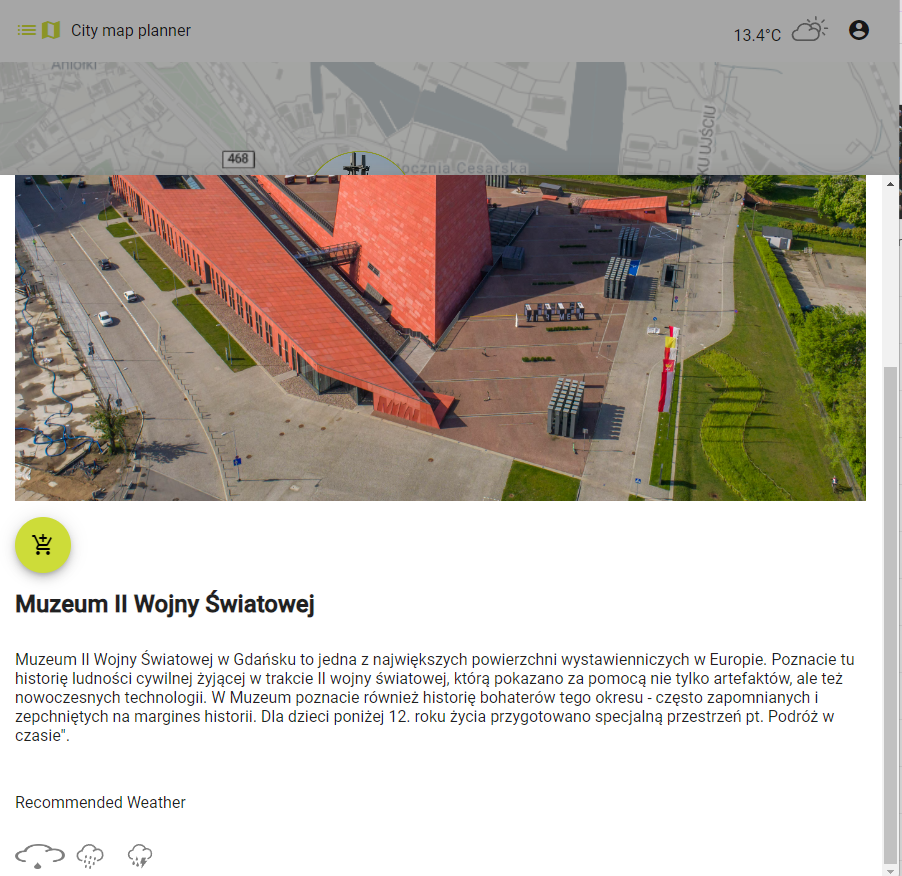
\includegraphics[width=1\textwidth]{attachments/atrakcjawidok-light}
    \caption{Widok pojedynczej atrakcji}
    \label{fig:mapawidok}
\end{figure}
\section{Widok koszyka}
\label{sec:koszyk}

Moduł koszyk~w~aplikacji pełni funkcję przechowywania~i~zarządzania wybranymi punktami zainteresowania (POI). 
Zaprojektowany z myślą~o~wygodzie użytkownika, widok koszyka umożliwia łatwe przeglądanie, modyfikowanie oraz usuwanie dodanych POI.

    \begin{figure}[H]
        \centering
        \includegraphics[width=1\textwidth]{attachments/koszyk}
        \caption{Widok koszyka}
        \label{fig:koszyk}
\end{figure}

\section{Widok kalendarza}
\label{sec:kalendarz}
Widok kalendarza~w~aplikacji sumuje wszystkie dodane atrakcje do koszyka, umożliwiając użytkownikowi planowanie wizyt~w~wybranych punktach zainteresowania (POI). 
Domyślnie kalendarz wyświetla trzy dni~w~zakresie godzinowym od 10:00 do 20:00.
Kalendarz automatycznie uwzględnia godziny otwarcia atrakcji, aby wskazać możliwe terminy wizyt. 
Każdej atrakcji przypisany jest domyślny czas zwiedzania, który można dostosować według indywidualnych potrzeb.


\begin{figure}[H]
        \centering
        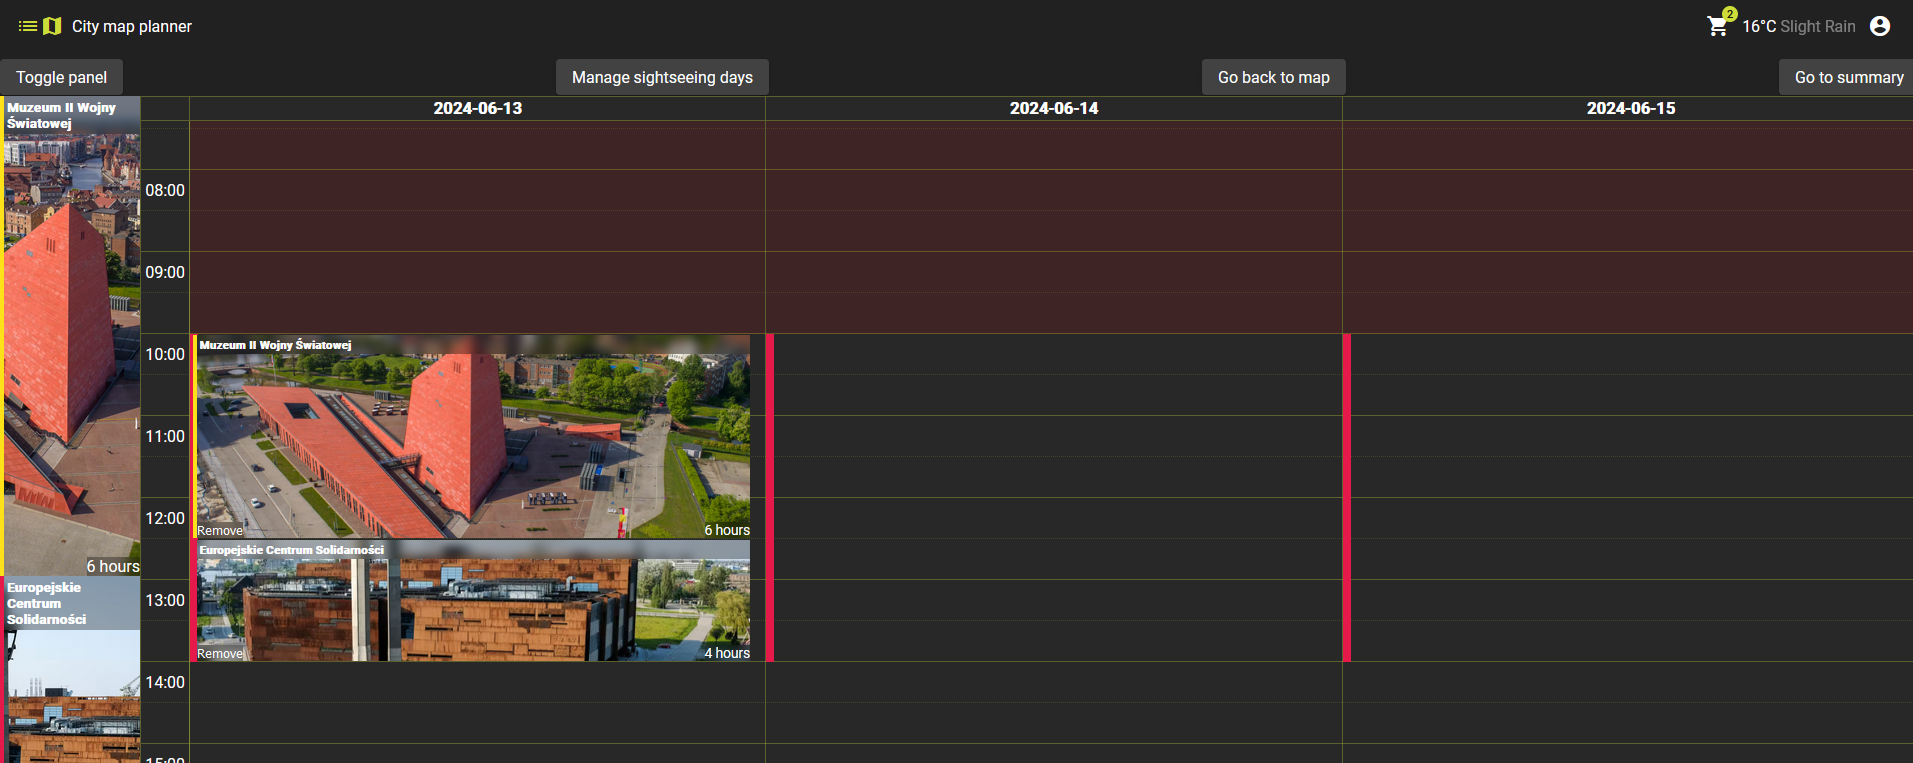
\includegraphics[width=1\textwidth]{attachments/kalendarz}
        \caption{Widok kalendarza}
        \label{fig:kalendarz}
\end{figure}
\begin{figure}[H]
    \centering
    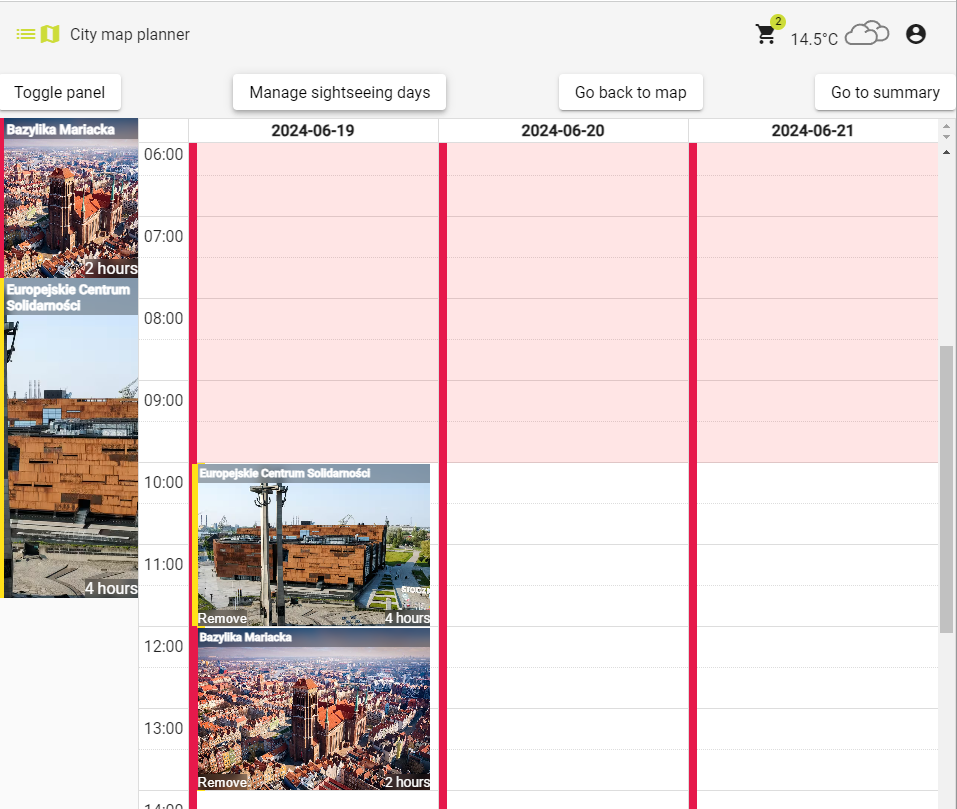
\includegraphics[width=1\textwidth]{attachments/kalendarz-light}
    \caption{Widok kalendarza jasny}
    \label{fig:kalendarz-light}
\end{figure}

\section{Widok podsumowania}
\label{sec:podsumowanie}
Widok podsumowania~w~aplikacji prezentuje wyznaczoną kolejność zwiedzania atrakcji na osi czasu. Umożliwia użytkownikowi łatwe śledzenie planu dnia
Na osi czasu wyświetlane są kolejne atrakcje~w~zaplanowanej kolejności.
Dzięki temu użytkownik może szybko~i~wygodnie ocenić, jak wygląda jego harmonogram ,
zwiedzania oraz upewnić się, że wszystkie planowane atrakcje są uwzględnione~w~odpowiednich przedziałach czasowych.

\begin{figure}[H]
    \centering
    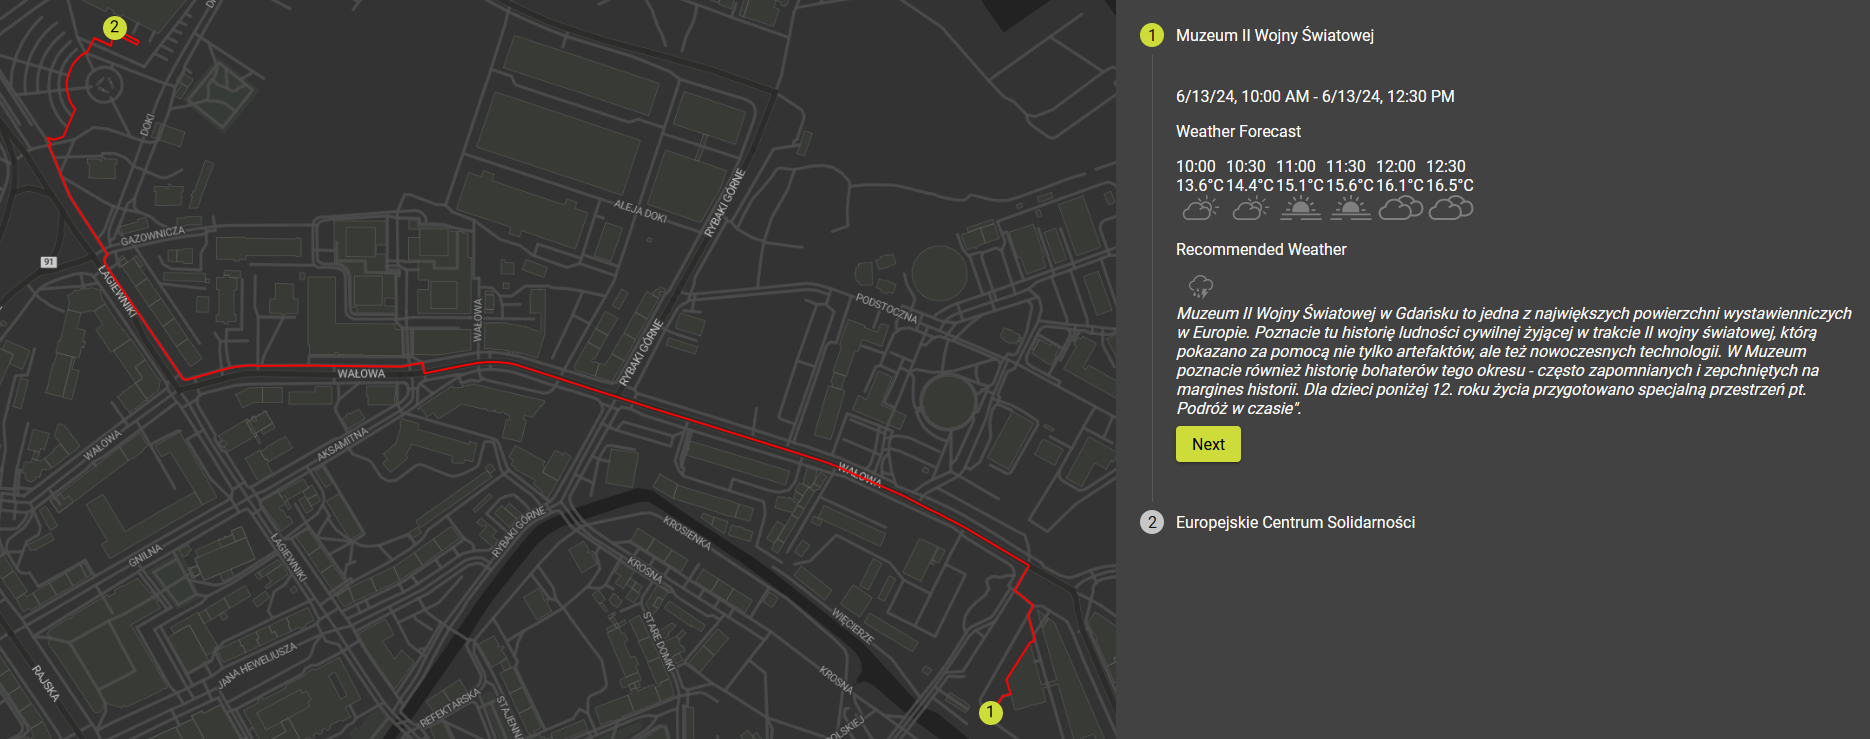
\includegraphics[width=1\textwidth]{attachments/podsumowanie}
    \caption{Widok podsumowanie}
    \label{fig:podsumowanie}
\end{figure}
\begin{figure}[H]
    \centering
    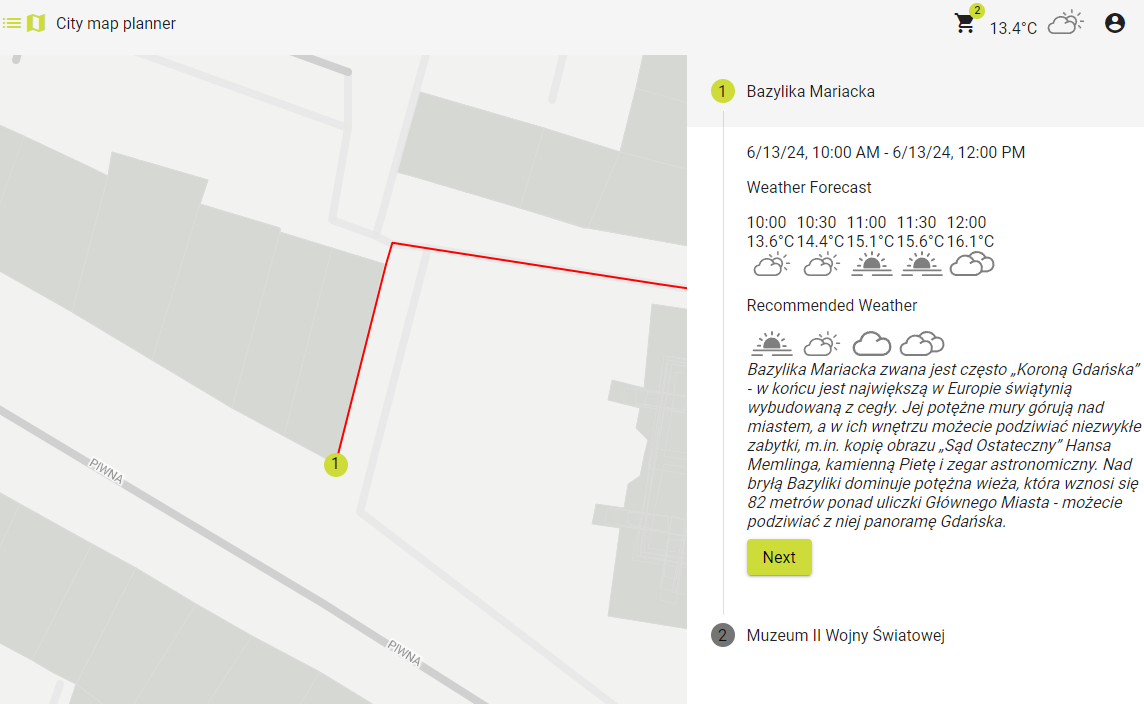
\includegraphics[width=1\textwidth]{attachments/podsumowanie-light}
    \caption{Widok podsumowanie wersja jasna}
    \label{fig:podsumowanie-light}
\end{figure}

\section{Widok Listy POI}
\label{sec:poilist}

Widok listy POI jest kluczowym narzędziem~w~aplikacji, które umożliwia użytkownikom 
efektywne przeglądanie~i~wybieranie interesujących atrakcji, co znacząco poprawia komfort~i~wygodę korzystania z aplikacji.
\begin{figure}[H]
    \centering
    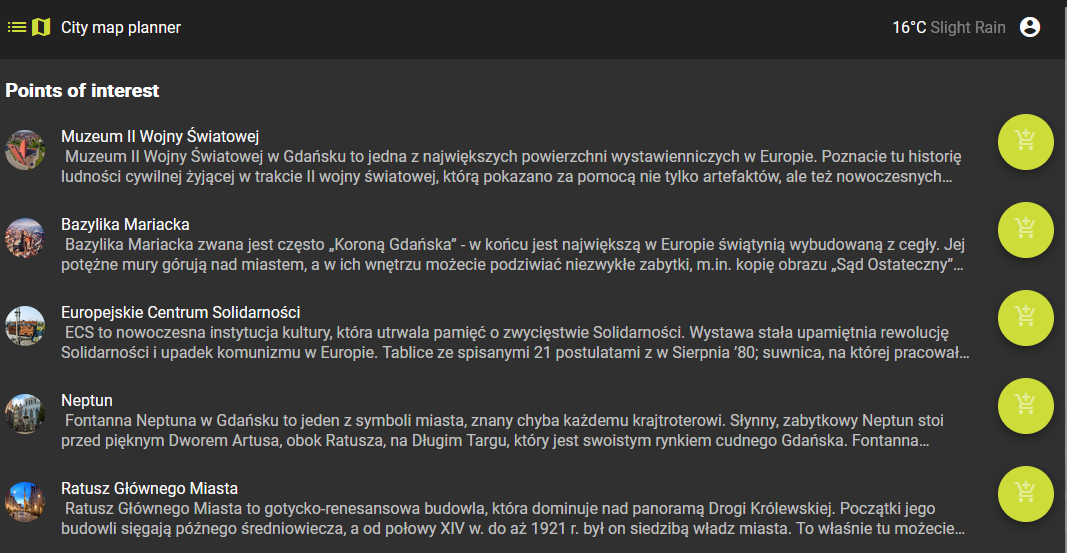
\includegraphics[width=1\textwidth]{attachments/poilist}
    \caption{Widok listy wszystkich dostępnych atrakcji}
    \label{fig:poilist}
\end{figure}

\section{Widok Logowania}
\label{sec:logowanie}

Widok logowania~w~aplikacji jest zaprojektowany, aby umożliwić użytkownikom łatwe~i~bezpieczne 
zarządzanie swoim kontem. Obejmuje on funkcje logowania, rejestracji oraz resetowania hasła.

\begin{figure}[H]
    \centering
    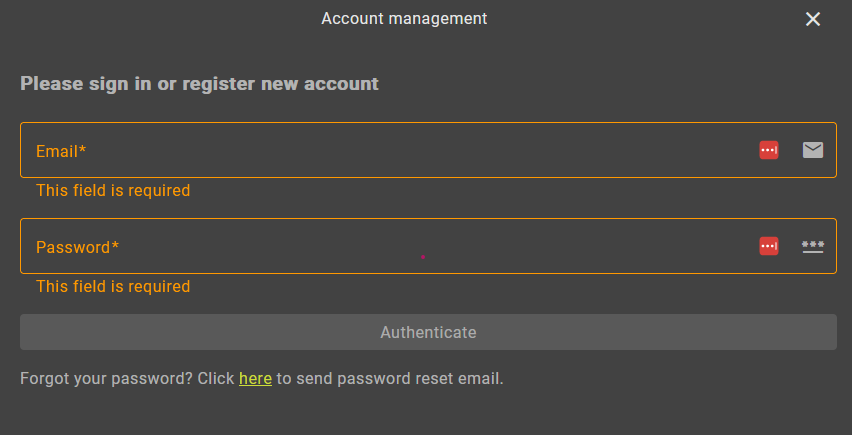
\includegraphics[width=1\textwidth]{attachments/logowanie}
    \caption{Widok panelu logowania}
    \label{fig:logowanie}
\end{figure}

\section{Widok zarządzania kontem użytkownika}
\label{sec:user}
Widok zarządzania kontem użytkownika~w~aplikacji zapewnia pełną kontrolę 
nad danymi~i~umożliwia wygodne zarządzanie kontem. Obejmuje funkcje wylogowania, usunięcia konta oraz zmiany danych.
\begin{figure}[H]
    \centering
    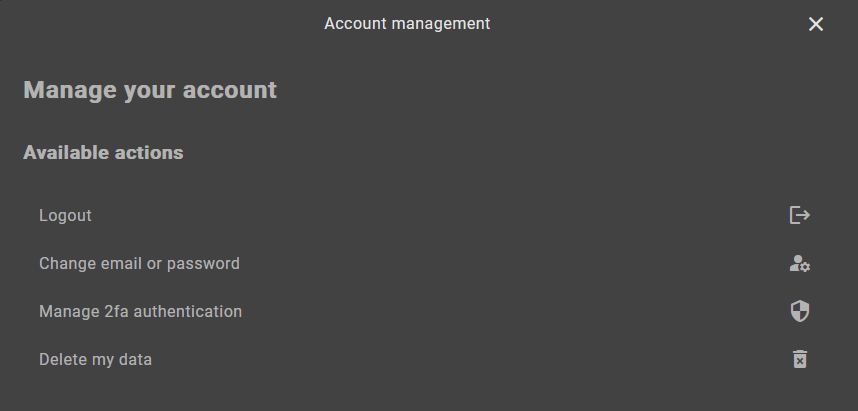
\includegraphics[width=1\textwidth]{attachments/user}
    \caption{Widok panelu zarządzania użytkownikiem}
    \label{fig:user}
\end{figure}

\section{Widok zarządzania wszystkimi POI}
\label{sec:manage}
Widok zarządzania wszystkimi punktami zainteresowania (POI) umożliwia dodawanie oraz modyfikowanie administratorowi 
szczegółowych informacjami~o~atrakcjach. Poniżej znajduje się opis poszczególnych pól~w~widoku:
\begin{itemize}
    \item Nazwa (name): Nazwa punktu zainteresowania, która identyfikuje daną atrakcję.
    \item Opis (description): Szczegółowy opis atrakcji, zawierający informacje~o~jej historii, znaczeniu~i~dostępnych aktywnościach.
    \item URL strony z godzinami otwarcia;
    \item XPath strony z godzinami otwarcia;
    \item URL strony z dniami wolnymi ;
    \item XPath strony z dniami wolnymi;
    \item  Preferowane kody WMO: Kody WMO (World Meteorological Organization), preferowane dla danego punktu zainteresowania, które mogą być użyte do określenia odpowiedniej pogody;
    \item  Sugerowany czas potrzebny na zwiedzanie atrakcji, dostosowany do typowego czasu trwania wizyty;
    \item Automatyczna aktualizacja godzin otwarcia na podstawie modelu sztucznej inteligencji.
\end{itemize}

Widok panelu dodawania punktów zainteresowania (POI)~w~aplikacji zapewnia administratorom pełen zestaw narzędzi do wprowadzania nowych atrakcji. 
Panel ten oferuje takie same możliwości jak widok arządzania wszystkimi POI, umożliwiając dokładne~i~szczegółowe wprowadzenie 
niezbędnych informacji~o~nowych punktach zainteresowania.


    \begin{figure}[H]
    \centering
    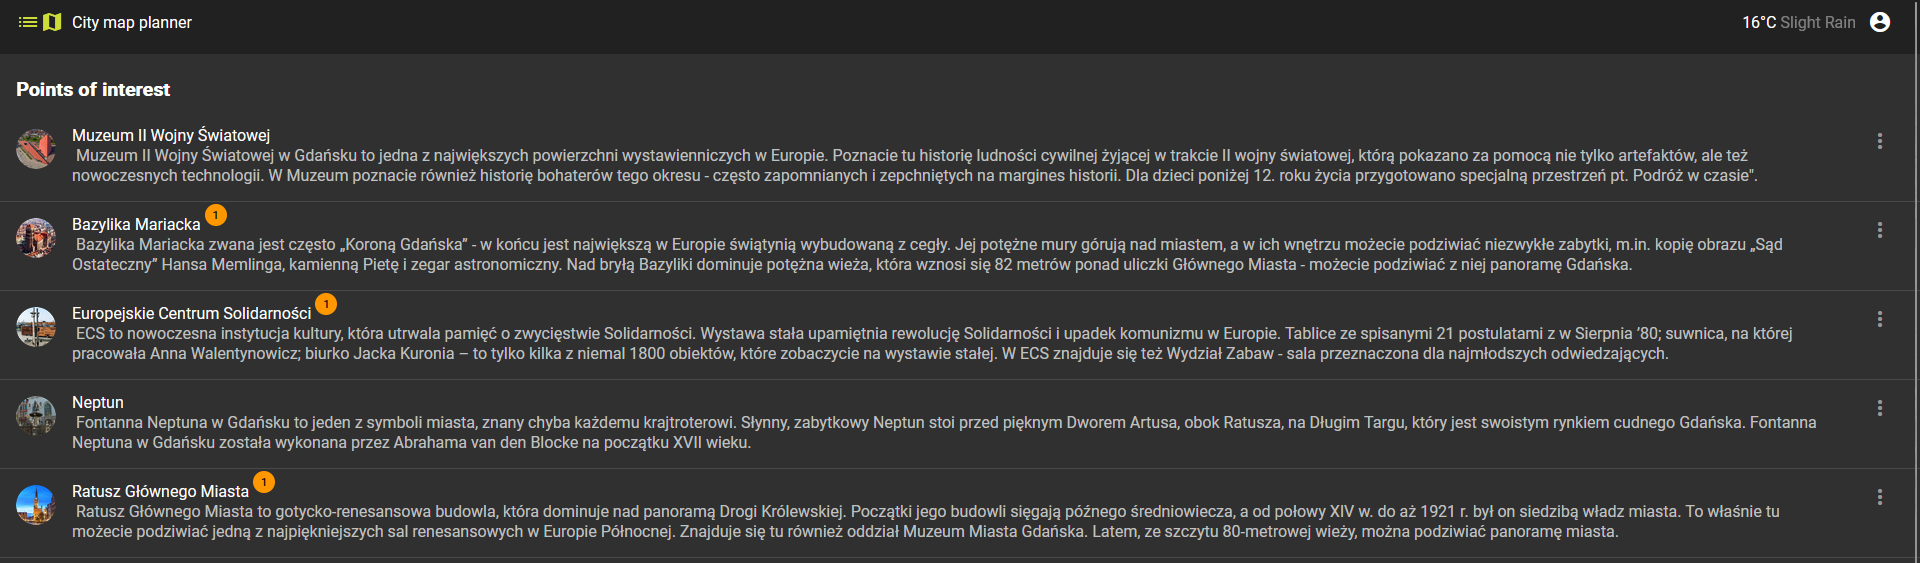
\includegraphics[width=1\textwidth]{attachments/poi-manage}
    \caption{Widok panelu zarządzania wszystkimi POI}
    \label{fig:poi-manage}
\end{figure}
\begin{figure}[H]
    \centering
    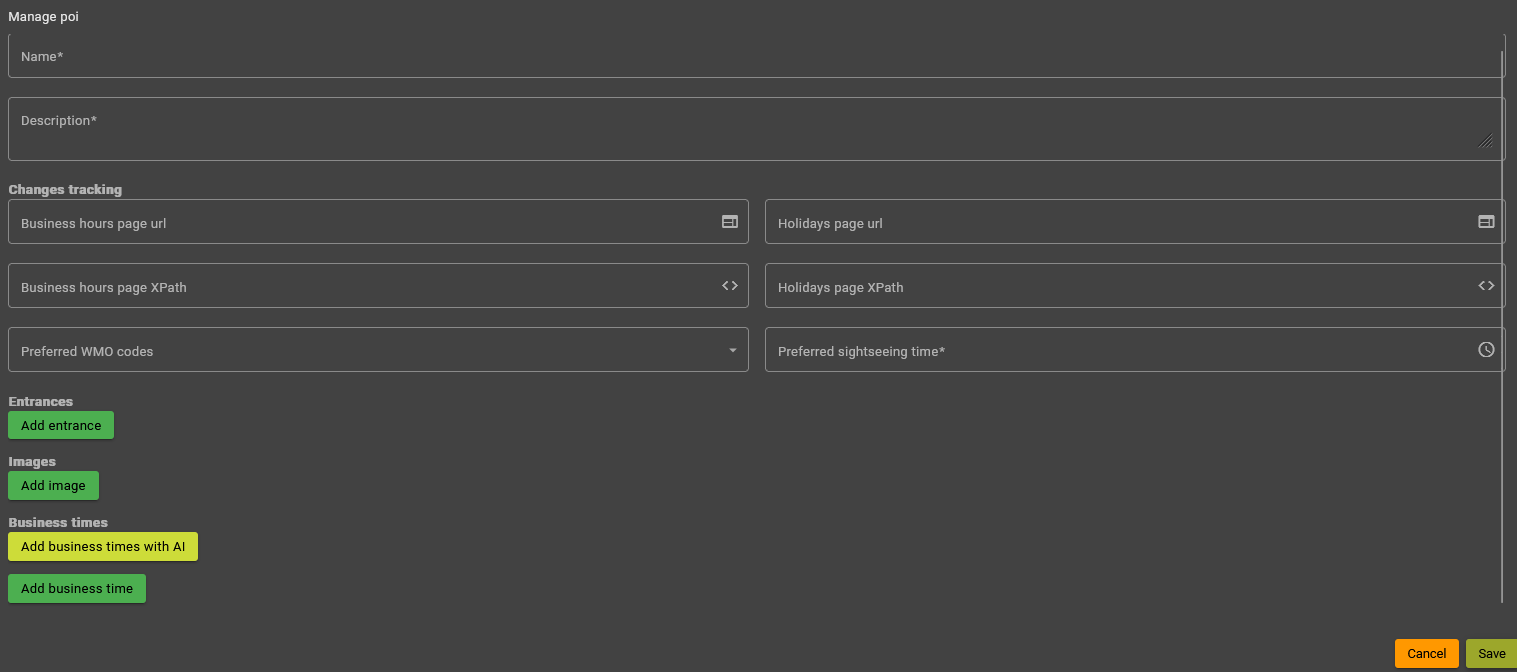
\includegraphics[width=1\textwidth]{attachments/addpoi}
    \caption{Widok panelu dodawania POI}
    \label{fig:ManageNofify}
\end{figure}

Dodatkowo, na stronie zarządzania POI znajduje się specjalna funkcja informująca~o~potrzebie sprawdzenia aktualności danych. 
Funkcja ta automatycznie monitoruje daty ostatnich modyfikacji~i~przypomina administratorom~o~konieczności weryfikacji~i~aktualizacji informacji~o~atrakcjach. 
Dzięki temu, dane prezentowane użytkownikom są zawsze aktualne~i~dokładne, co zapewnia lepsze doświadczenie użytkownika oraz zwiększa zaufanie do aplikacji.
\begin{figure}[H]
    \centering
    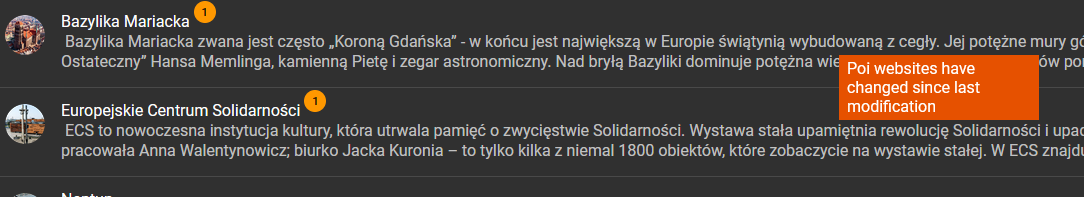
\includegraphics[width=1\textwidth]{attachments/poi-notify}
    \caption{Informacja~o~potrzebie sprawdzenia aktualności danych}
    \label{fig:ManageNofify}
\end{figure}
